\begin{multicols}{3}[\section{DECT - Digital Enhanced Cordless Telecommunications}]

\rhead{Simon Retzmann, Thomas Schaffroth}
\lfoot{08.05.2016}

\newrefsegment

\begin{tabular}{p{2,1 cm}p{2.7 cm}}
\textbf{Steckbrief}& \\
\end{tabular}
\rowcolors{1}{\topicolor!20}{}
\begin{tabular}{p{2,1 cm}p{2.7 cm}}
      Einsatz seit & 1994\\
      Frequenz"-bereich  & \SI{1880}-\SI{1900}{\mega\hertz} (Europa)\\
      Datenrate & \SI{800}{kbit/s}\\
      Verbreitung & Weltweit\\
      Reichweite & \SI{30}{\metre}-\SI{50}{\metre}\\
      Modulation & FDMA, TDMA\\
      Sendeleistung & 250 mW\\
      Verschlüsselung & AES-Verschlüsselung mit 128 Bit\\
\end{tabular}
\par
%Source http://www.fh-bingen.de/fileadmin/user_upload/Lehrende/Kilsch_Dieter/internet/projekte/TedoSchStiUnits.pdf -> Seite 9 findet ihr alle verwendbaren Einheiten, wie:
%\SI{Zahl}{\mega\hertz} oder \SI{Zahl}{\mili\metre}
%Ich weiß ehrlich gesagt nicht welche Einheiten ihr im Text genau braucht, aber in dem Dokument und mit obigen Beispiel sollte es umsetzbar ein.
\subsection*{Überblick}
\begin{wrapfigure}{r}{0.4\linewidth}
  \vspace{-20pt}
  \begin{center}
  	\hspace{-20pt}
    
\includegraphics[width=0.7\linewidth]{Kapitel/DECT/Grafiken/logo.png}
  \end{center}
  \vspace{-15pt}
\end{wrapfigure}
Der Standard \textit{DECT} (\textbf{D}igital \textbf{E}nhanced \textbf{C}ordless \textbf{T}elecommunications) ist eine universelle Kurzstrecken-Funktechnik für die Telekommunikation. Im Bereich der schnurlosen Sprachübertragung hat sich \textit{DECT}weltweit etabliert.
Für eine reibungslose Interaktion mit verschiedenen Telefonnetzen nutzt DECT definierte Zugriffsprotokolle und sogenannten Access Profiles; dadurch kann zum Beispiel eine \textit{ISDN} (\textbf{I}ntegrated \textbf{S}ervices \textbf{D}igital \textbf{N}etwork) oder \textit{GSM} (\textbf{G}lobal \textbf{S}ystem for \textbf{M}obile) Konnektivität hergestellt werden. 
Mithilfe der Protokollstruktur können verschiedene Basisstationen zu einem Telefonnetz zusammengeschaltet werden. Unterstützt werden Ein- und Mehrzellensysteme mit gleitendem Übergang zwischen den Zellen, wodurch sich ein \textit{DECT}-Netz über zum Beispiel größere Firmengelände aufbauen lässt.
\cite{dect.1}

\subsection*{Technische Erläuterung}

\subsubsection*{Eigenschaften}
In einer internationalen Übereinkunft wurde von der \textit{ETSI} im \textit{DECT} Standard festgelegt, dass \textit{DECT} abhör- und ausfallsicher ist. Außerdem soll nur ein geringes Frequenzband genutzt werden, wodurch Frequenzen eingespart werden. Des Weiteren soll \textit{DECT} mit einer hohen Qualität in der Sprachübertragung universell einsetzbar sein. Ein nahtloser Übergang zwischen den Funkzellen ist dabei zu gewährleisten, damit wie bereits erwähnt ein \textit{DECT}-Netz für ein großes Firmengelände aufgebaut werden kann.

\textit{DECT} bietet außerdem:
\begin{itemize}
	\item  ein exklusives Frequenzband für den Betrieb
	\item Optimierung auf gleichbleibende Verbindungsqualität und minimale Verzögerung
	\item hohe Reichweite
	\item geringen Stromverbrauch
	\item geringe Kosten für Endgeräte
	\item Telefonie-Leistungsmerkmale:
	\begin{itemize}
		\item gleichzeitiger Betrieb mehrerer Mobilteile
		\item gebührenfreie interne Gespräche
		\item Mobilteile sind an mehreren Basisstationen nutzbar
		\item herstellerunabhängige Nutzung von Mobilteilen an verschiedenen Basisstationen
		\item Handover (automatischer Wechsel der Basisstation)
	\end{itemize}
\end{itemize}
\cite{dect.1}

\subsubsection*{Fixed Part und Portable Part}
Bei \textit{DECT} ist der Fachbegriff für die  Basisstation der Fixed Part; dieser wechselt seinen Standort nicht. Portable Part ist das Handgerät also das eigentliche schnurlose Telefon des \textit{DECT}-Systems. 
Der Fixed Part übernimmt die Vermittlung der Gespräche und stellt dem Benutzer über das Portable Part die Leistungsmerkmale und die Schnittstelle in das leitungsvermittelte Telefonnetz zur Verfügung. \cite{dect.1}

\subsubsection*{Strahlung der \textit{DECT}-Telefone}
Die schnurlosen Telefone haben einen Eco-Modus, der das Telefon automatisch in einen Betriebsmodus mit geringen elektromagnetischen Feldern versetzt. Dieser wurde aufgrund von Kundennachfragen in fast allen \textit{DECT}-Telefonen implementiert, denn nach wissenschaftlicher Erkenntnis geht von \textit{DECT} keine Gefahr aus.
Im Eco-Modus sendet der Fixed Part (die Basistation) mit der Leistung, die notwendig ist, um das am weitesten entfernte Mobilteil zu erreichen. Das bedeutet je näher sich der Portable Part am Fixed Part befindet, desto geringer ist die Funkleistung. Bei einem Portable Part bedeutet es, dass die Funkleistung bei Annäherung an den Fixed Part verringert wird. Bei mehreren Portable Parts müssen sich alle Geräte dem Fixed Part nähern, um diesen Effekt zu erreichen. \cite{dect.1}

\subsubsection*{Übertragung}
Für die Übertragung bei \textit{DECT} wird das Modulationsverfahren GFSK (\textbf{G}ausian \textbf{F}requency \textbf{S}hift \textbf{K}eying) eingesetzt, da hier effiziente Verstärker zur Reduktion des Stromverbrauchs und der Wärmeentwicklung genutzt werden können.
Die Portable Parts überprüfen ständig die Träger zwischen \SI{1880}-\SI{1900}{\mega\hertz} (10 HF-Kanäle mit \SI{1728}{\kilo\hertz} Abstand). Verwendet wird der Träger mit dem besten Empfangsergebnis. Dieses Verfahren wird Dynamic Channel Selection/Allocation genannt, welches die Störanfälligkeit der Übertragung senkt und gleichzeitig die Sprachqualität erhöht. \cite{dect.1}

\begin{Figure}
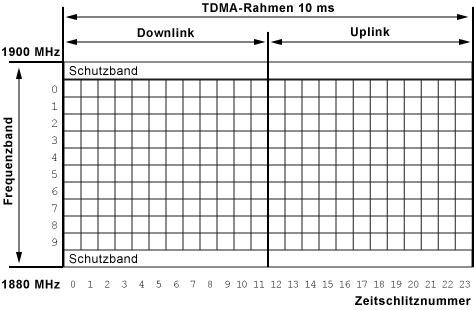
\includegraphics[width=\linewidth]{Kapitel/DECT/Grafiken/frequenzband.png}
\captionof{figure}{Frequenzband von \textit{DECT} \cite{dect.1}}
\label{fig:dect.frequenzband}
\end{Figure}
Für die Modulation wird das Frequenzband in 10 Frequenzträger unterteilt, jeweils oben und unten befindet sich ein Schutzband, um Störungen durch Überlappungen mit anderen Frequenzen zu reduzieren. 

Jeder Frequenzträger wird in 24 Zeitschlitze unterteilt, jeweils 12 Zeitschlitze sind für die Verbindung vom Fixed Part zum Portable Part und umgekehrt reserviert. Die Dauer eines Frames (24 Zeitschlitze) sind 10ms.
Das Nutzsignal wird mit der GFSK Modulation übertragen und bietet eine Bandbreite von 32 kBit/s und bietet damit eine dem Festnetz ähnliche Sprachqualität.

Für die Sprachübertragung werden die Zeitschlitze symmetrisch aufgeteilt, bei Datenübertragungen asymmetrisch mit Bündelung mehrerer Kanäle. Bis zu 23 Kanäle lassen sich bündeln, denn es muss noch mindestens ein Kanal für die andere Richtung zur Verfügung stehen \cite{dect.1}.
Die Frequenzmodulation kann allerdings auch mit 4PSK, 8PSK, 16QAM und 64QAM realisiert werden.

\subsubsection*{\textit{DECT} ULE (Ultra-low Energy)}
Bei \textit{DECT} Ultra-low Energy geht es um die Senkung des Energieverbrauches; die Teilnehmer werden dabei in einen zyklischen Tiefschlaf versetzt. Durch ein Ereignis können die Teilnehmer aus dem Tiefschlaf geholt werden. Kurze Tiefschlafphasen erhöhen allerdings nicht signifikant die Akkulaufzeit, daher wählt man die Pausen möglichst lange, jedoch nicht länger als 20 Sekunden. \cite{dect.1}

\subsubsection*{Datenübertragungen mit \textit{DECT}}
\textit{DECT} wurde für die schnurlose Sprachübertragung entwickelt, entsprechend ist \textit{DECT} zur Datenübertragung nur mit Einschränkungen nutzbar. Die Daten können mit 24 kBit/s pro Kanal übertragen werden. 23 Kanäle lassen sich bündeln, sodass eine Übertragung von 552 kBit/s erreicht werden kann. Üblicherweise können \textit{DECT}-Datenübertragungsgeräte nur 128 kBit/s übertragen. Mithilfe des DMAP (\textbf{D}ECT \textbf{M}ultimedia \textbf{A}ccess \textbf{P}rofile) können die vorhandenen 552 kBit/s voll ausgenutzt werden und für ein schnurloses Netzwerk auf Basis von \textit{DECT} verwendet werden. Für die breitbandige Datenübertragung ist dies allerdings nicht ausreichend, weshalb der Nachfolge-Standard CAT-iq entwickelt wurde. \cite{dect.1}

\subsubsection*{GAP - Generic Access Profile}
Das bekannteste \textit{DECT}-Zugriffsprofil ist das GAP (\textbf{G}eneric \textbf{A}ccess \textbf{P}rofile), welches bereits 1994 von \textit{ETSI} spezifiziert wurde. GAP ermöglicht die Zusammenarbeit zwischen \textit{DECT}-Geräten unterschiedlicher Hersteller. Alle GAP-kompatiblen Portable Parts lassen sich herstellerunabhängig mit den Telefon-Grundfunktionen an allen GAP-kompatiblen Fixed Parts betreiben. GAP garantiert zwar die Kompatibilität der Mobilteile, jedoch bezieht sich das nur auf die reine Telefonie. Funktionen wie der Anrufbeantworter oder das Telefonbuch funktionieren gegebenenfalls nicht. \cite{dect.4,dect.1}

\end{multicols}
\newpage
\section*{Historische Entwicklung}
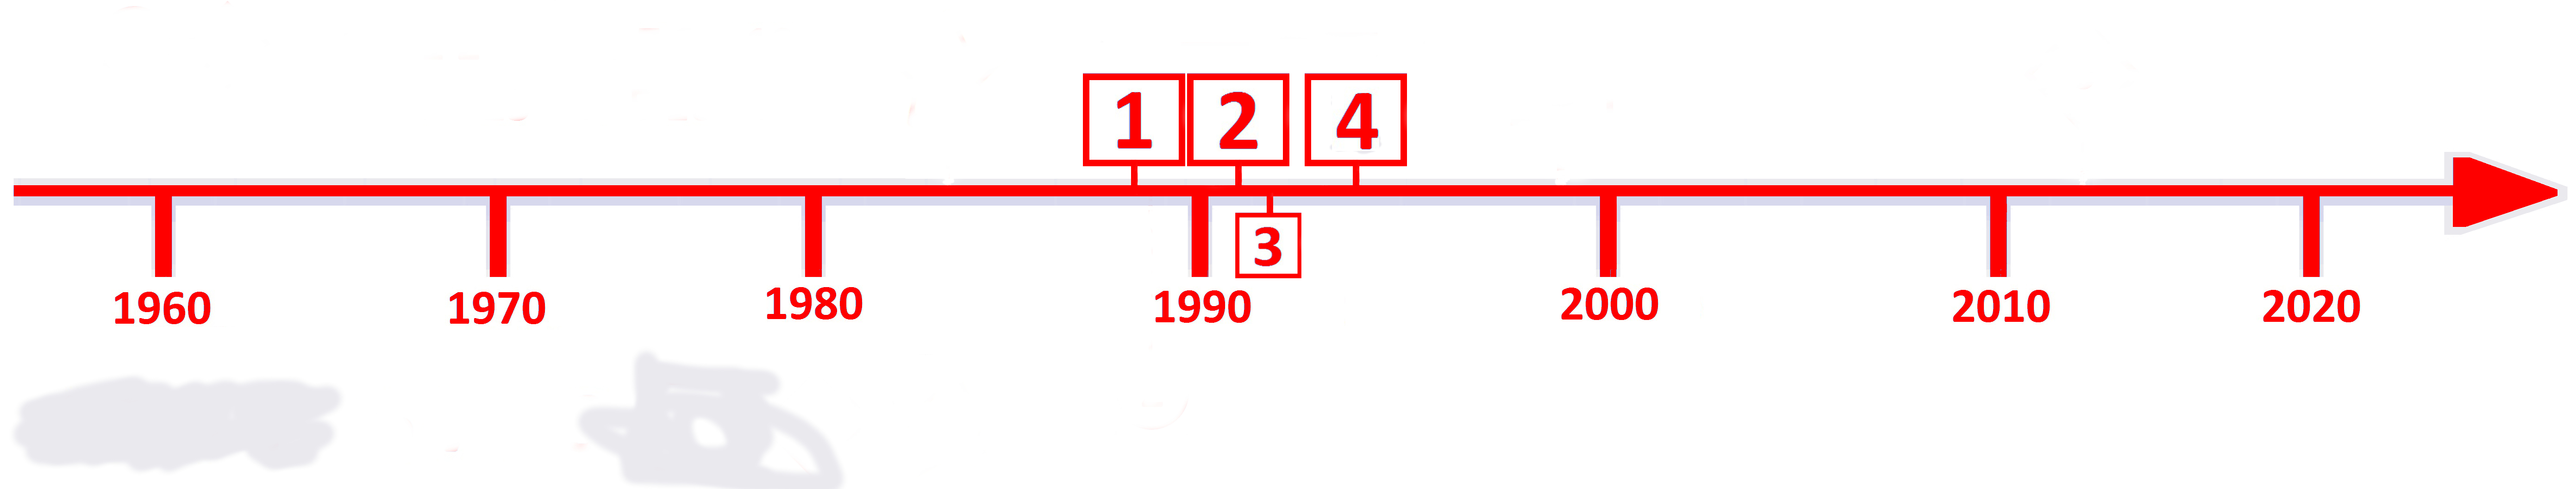
\includegraphics[width=\textwidth]{Kapitel/DECT/Grafiken/ZeitstrahlDect}
\par
\noindent
\rowcolors{2}{}{\topicolor!20}
\begin{tabular}{p{0.5 cm}p{1.5 cm}p{15.55 cm}}
	Nr. & Datum & Entwicklungsschritte~\cite{dect.9}\\
	1 & 1988 & Aufgabe der ETSI (European Telecommunications Standards Institute) einen europäischen Standard für digitale Schnurlos-Telefone und -Telefonanlagen zu definieren.\\
	2 & Juni 1991 & Die wichtigsten Teile des Standards gehen in die öffentliche Kommentierung.\\
	3 & 1992 & Erste DECT-Geräte sind im Handel erhältlich.\\
	4 & 1994  & Definition des Generic Access Profiles (\textbf{GAP}), das es ermöglichte Geräte verschiedener Hersteller miteinander zu kombinieren.\\
\end{tabular}
\par
\begin{multicols}{3}

\subsubsection*{IAP - ISDN Access Networking Profile}
Mithilfe dieser Spezifikation ist ein \textit{DECT}-Telefon in der Lage ISDN-Komfortmerkmale aus dem Telefonie-Bereich zu nutzen. Zum Beispiel gehört die Rufnummernanzeige, Anklopfen, Dreierkonferenz oder Rufumleitung dazu. Dieses Profil ist weit verbreitet und fast alle \textit{DECT}-Telefone beherrschen dieses Profil. \cite{dect.1}

\subsubsection*{GIP - GSM Interworking Profile}
Dieses Zugriffsprotokoll regelt die Zusammenarbeit mit digitalen Mobilfunknetzen, die dem GSM-Standard entsprechen (für UMTS existiert auch ein Profil). Mithilfe von Dualmode-Handys lässt sich eine Kombination aus Mobilfunknetz und Festnetz erstellen. Dadurch lässt sich zuhause das Festnetz nutzen und unterwegs das Mobilfunknetz. Unterstützt der Netzbetreiber (Mobilfunk und Festnetz) entsprechende Routing-Techniken, kann für beide Netze dieselbe Telefonnummer angeboten werden. Geräte mit dieser Funktionalität sind jedoch nicht weit verbreitet. \cite{dect.1}
\subsubsection*{\textit{DECT} CAT-iq}
\textit{DECT CAT-iq} (\textbf{C}ordless \textbf{A}dvanced \textbf{T}echnology - \textbf{i}nternet and \textbf{q}uality) soll die Konvergenz von Sprach- und Breitbandübertragungen erhöhen. Neben der Sprachübertragung in Hifi-Qualität können auch Internet-Dienste eingebunden werden. Mithilfe von \textit{CAT-iq} wird das \textit{DECT}-Gerät IP-fähig.

Ermöglicht wird damit unter anderem:
\begin{itemize}
\item Musik-Streaming
\item Informationsanzeigen und -dienste aus dem Internet
\item Instant-Messaging 
\item Home-Management-Funktionen
\end{itemize}

Eine Weiterentwicklung von \textit{DECT} für Datenübertragungen wirkt auf den ersten Blick erst einmal überflüssig. Es stellt sich die Frage warum etwas neu entwickelt werden sollte, wenn doch zur Übertragung der Daten die WLAN-Funktechnik genutzt werden könnte. Allerdings war WLAN (\textbf{W}ireless \textbf{LAN}) lange nicht als Schnurlostechnik für Telefone geeignet, denn die für die Datenkommunikation ausgelegte WLAN-Technik verbrauchte sehr viel Rechenleistung und hat einen entsprechenden Energieverbrauch. Außerdem funkt WLAN im freien ISM-Band, wo sich auch noch andere Funkanwendungen befinden, weshalb Störungen nicht ausgeschlossen sind. \textit{DECT} hat den Vorteil ein eigenes Frequenzspektrum mit einer höheren Reichweite zu haben. \textit{CAT-iq} nutzt den \textit{DECT}-Frequenzbereich und ist zum bisherigen etablierten \textit{DECT}-Standard abwärtskompatibel. \cite{dect.3}

\subsection*{Einsatz}
\textit{DECT} ist als \textit{ETSI}-Standard für Kurzstrecken-Funktechnik entwickelt worden und kann für viele Anwendungen in der ganzen Welt in unlizensierten Frequenzbereichen genutzt werden. \textit{DECT} ist für Telefonie (PSTN und VoIP) und Datenübertragung mit einer Reichweite bis zu 500 Metern entwickelt.

Seit Beginn wurden mehr als 820 Millionen Geräte hergestellt, jährlich kommen ca. 100 Millionen Geräte dazu. \textit{DECT} dominiert den kabellosen Sprachübertragungssektor mit einem Marktanteil von 73\% aller kabellosen Technologien (inklusive analogen und proprietären). \textit{DECT} erhält mehr Marktanteil durch den Austausch von alten analogen Technologien, verliert aber auch Marktanteile durch die digitalen Technologien basierend auf IEEE 802.11. Die geringen Kosten von \textit{DECT} Chipsätzen durch Massenproduktion erlauben den Austausch von fest verkabelten Telefonen.

\textit{DECT} wurde initial für Europa entwickelt, ist jedoch mittlerweile in über 110 Ländern adoptiert worden. Die Vereinigten Staaten von Amerika haben sich gegenüber \textit{DECT} über eine \textit{FCC} (\textbf{F}ederal \textbf{C}ommunications \textbf{M}ission) Entscheidung 2005 geöffnet und sind mit der wichtigste Markt hinsichtlich des Wachstums. Japan hat sich vor kurzem auch \textit{DECT} geöffnet, wo der Markt noch traditionell von \textit{The Personal Handyphone System} (\textbf{PHS}) dominiert wird.

Seit 2010 haben viele Betreiber in Europa ihre Telefonnetze auf IP-Netze umgestellt, damit geht eine qualitative Verbesserung der Sprachqualität einher. Statt bisher \SI{3.1}{\kilo\hertz} soll mindestens das Doppelte zur Verfügung stehen. Viele Endgeräte unterstützen  diesen sogenannten HD-Sound bereits.

Neuerungen:
Parallel zur Telefonie können noch weitere Daten wie z.B. ein externes Adressbuch, Webradio oder Ähnliches übertragen werden.
\cite{dect.3,dect.5}
\subsection*{Ausblick}
Innerhalb von Europa sind folgende Frequenzen für \textit{DECT} reserviert:
\begin{itemize}
\item \SI{1900}-\SI{1920}{\mega\hertz} (geteilt mit UTRAN TDD)
\item \SI{1920}-\SI{1980}{\mega\hertz} (geteilt mit dem Uplink von UTRAN FDD)
\item \SI{2010}-\SI{2025}{\mega\hertz} (vorgesehen für die potentielle Erweiterung von IMT-2000, noch nicht genutzt)
\end{itemize} 

\subsubsection*{Konkurrenz Voice-over-WLAN (VoWLAN)}
WLAN wurde nicht für die Sprachübertragung ausgelegt, jedoch wird mit dem Standard IEEE 802.11e Voice-over-WLAN (\textbf{VoWLAN}) die Sprachübertragung ermöglicht.

\textit{DECT} ist für Sprachkommunikation ausgelegt und dank des modularen Aufbaus lassen sich \textit{DECT}-Netze bei Bedarf mit weiteren Basisstationen erweitern. Durch nahtloses Handover wird eine ständige Konnektivität gewährleistet.

Bei VoWLAN existiert gerade bei Unternehmen in der Regel bereits eine Infrastruktur, weshalb Kosten gespart werden können, da nicht ein weiteres Funknetz aufgebaut werden muss. Allerdings haben \textit{DECT} Geräte durch einen geringeren Energieverbrauch als VoWLAN-Geräte eine längere Akkulaufzeit .
Letztendlich hängt die Entscheidung zwischen \textit{DECT} und VoWLAN vor allem von der bestehenden Infrastruktur ab. Wird diese allerdings neu aufgebaut, dann ist es in der Regel günstiger VoWLAN zu nutzen, da keine zwei Infrastrukturen aufgebaut werden müssen. Diese Kostenersparnis wird für viele relevant sein, weshalb \textit{DECT} eventuell in Zukunft vom Markt verschwinden könnte. WLAN entwickelt sich damit immer mehr zu einer universellen Standard-Infrastruktur. 

Für den Heimanwendungsbereich bietet zum Beispiel die FritzBox in den neueren Modellen mehrere Möglichkeiten. Der \textit{DECT} Standard ist implementiert, jedoch wird auch eine App für Smartphones zur Verfügung gestellt mit der man mit seinem Smartphone über WLAN telefonieren kann. 
\cite{dect.6,dect.7,dect.8}

\printbibliography[segment=1,heading=subbibliography]
\end{multicols}
\newpage
